\documentclass{../../slides-style}

\slidetitle{Автоматы и лексический анализ}{14.03.2026}

\begin{document}
    
    \begin{frame}[plain]
        \titlepage
    \end{frame}

    \section{Летучка}

    \begin{frame}
        \begin{center}
            \LARGE

            \structure{Летучка!}

            \vspace{1em}

            \Large
            Доставайте листочки и ручки
        \end{center}
    \end{frame}

    \begin{frame}{Летучка}
        \begin{enumerate}
            \item Дана матрица инцидентности графа $M$. Представьте этот граф визуально в виде узлов и дуг.
            $$
            M = \begin{pmatrix}
            1 & 0 & 0 & 0 & -1 \\
            -1 & -1 & 1 & 0 & 0 \\
            0 & 0 & -1 & -1 & 0 \\
            0 & 1 & 0 & 1 & 1
            \end{pmatrix}
            $$
            \item Дан граф $G = (V, E)$. Какова временная асимптотическая сложность алгоритма поиска в ширину (BFS) в худшем случае?
            
            \item Реализуйте функцию \mintinline{c}|void neighbors(int v, int size, int** graph)|,\\
            которая по матрице смежности и номеру вершины выводит на консоль все смежные вершины.
        \end{enumerate}
    \end{frame}

    \section{Работа компилятора}

    \begin{frame}{Напоминание о процессе компиляции кода на C}
        \begin{center}
            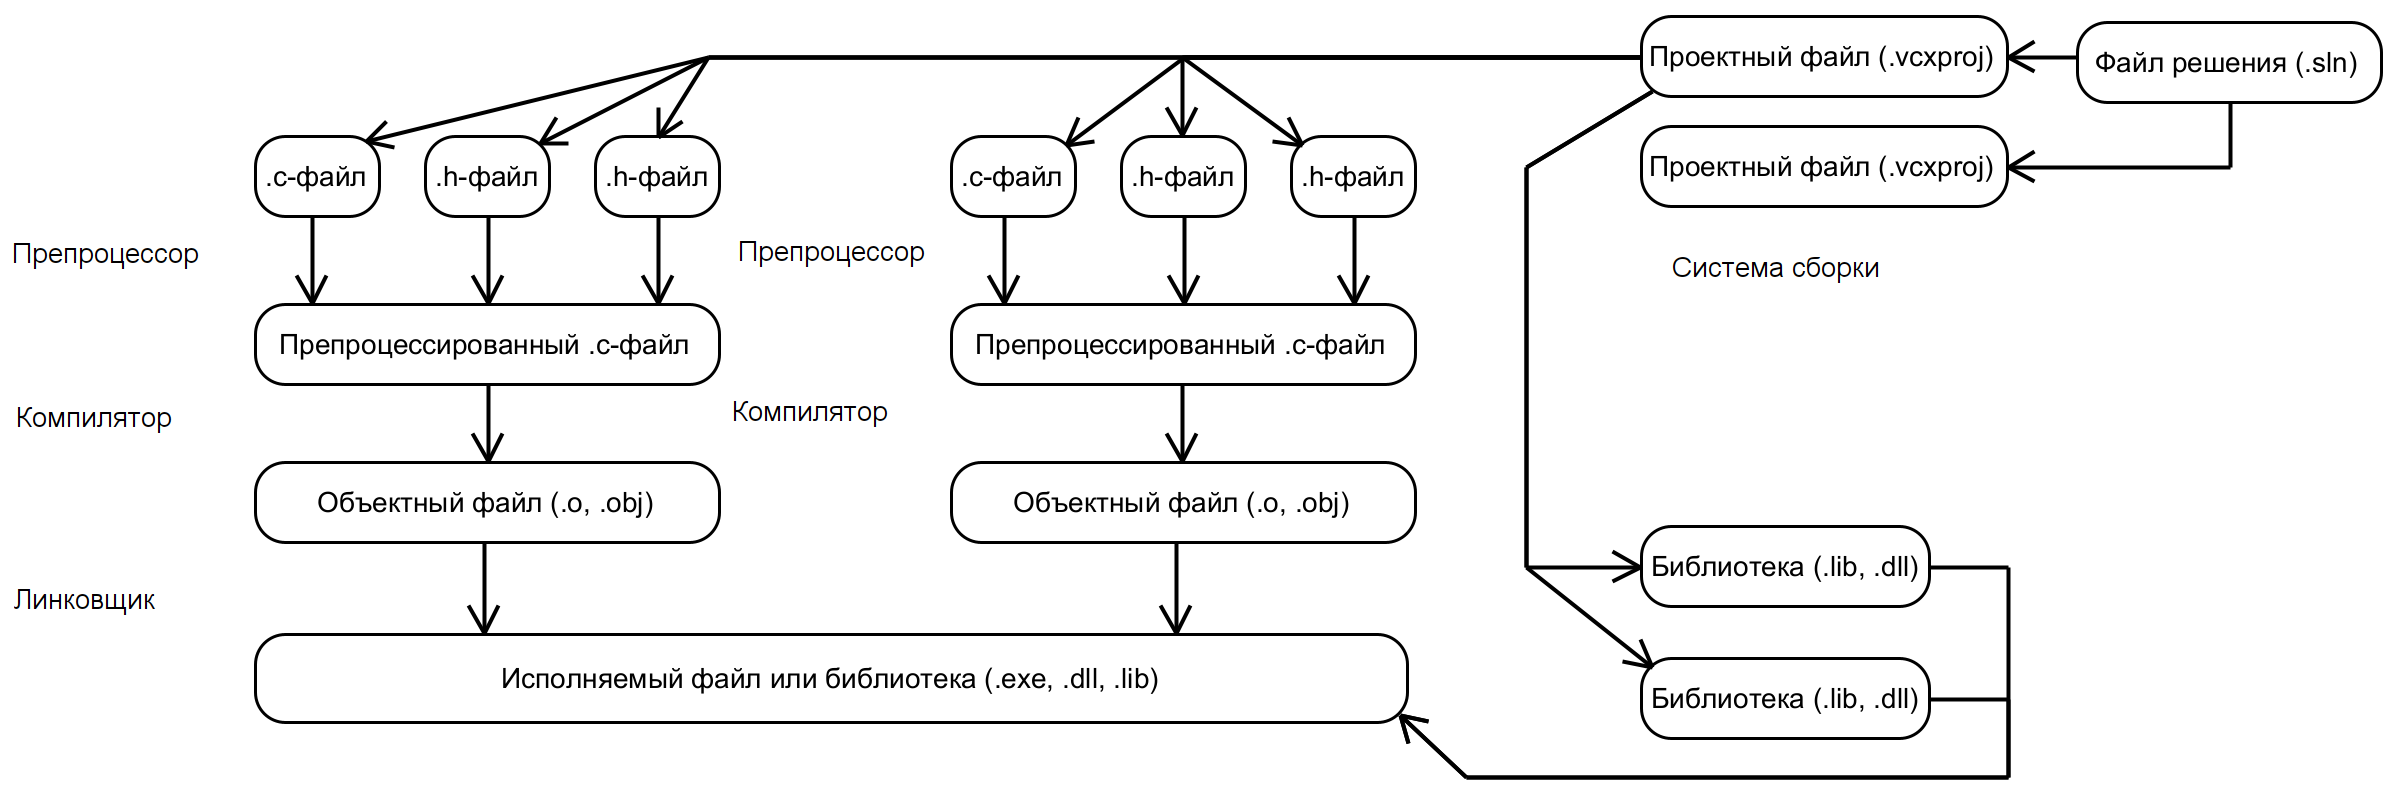
\includegraphics[height=0.4\textheight]{compilation.png}
        \end{center}
    \end{frame}

    \begin{frame}{Фазы компилятора}
        \begin{center}
            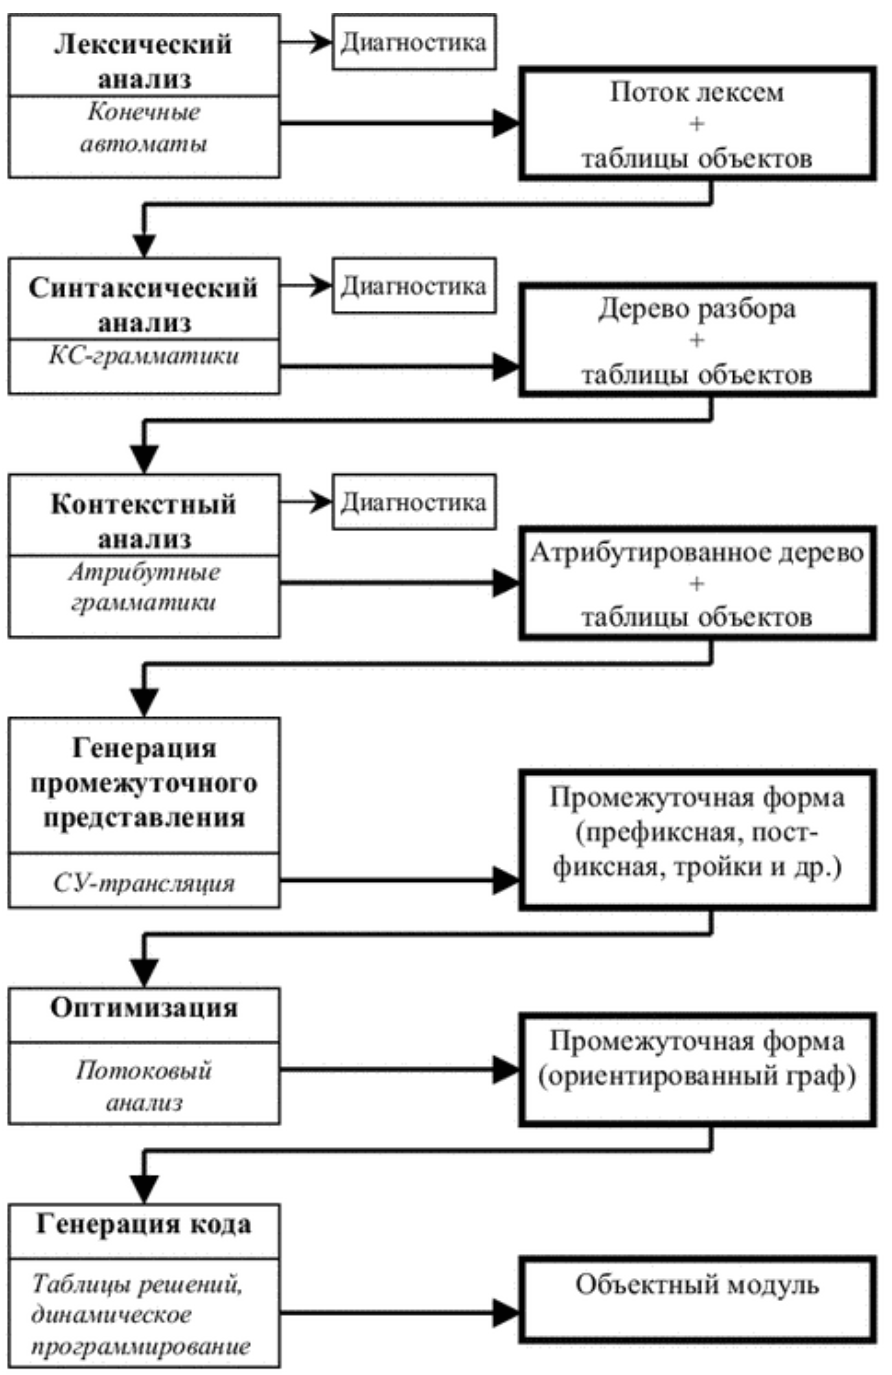
\includegraphics[height=0.8\textheight]{compilerPhases.png}
        \end{center}
    \end{frame}

    \begin{frame}{Лексический анализ}
        \begin{outline}
            \1 Преобразование потока символов в поток токенов
            \1 Например, \mintinline{text}|position := initial + rate * 60|
                \2 Идентификатор position
                \2 Символ присвоения
                \2 Идентификатор initial
                \2 Знак сложения
                \2 Идентификатор rate
                \2 Знак умножения
                \2 Число 60
            \1 Токен представляется в виде структуры из типа токена и его значения
        \end{outline}
    \end{frame}

    \section{Формальные языки}

    \begin{frame}{Формальные языки, определения}
        \begin{outline}
            \1 Алфавит --- произвольное множество. Элементы множества называются \textit{символами} алфавита
            \1 Строка (она же \textit{цепочка}) --- конечная последовательность символов из алфавита
            \1 Длина строки $s$ (обозначается как $\lvert{s}\rvert$) --- количество символов в строке
            \1 Пустая строка ($\epsilon$) --- строка, которая не содержит символов
            \1 Конкатенация строк --- две строки, записанные друг за другом
            \1 Язык --- множество строк. Например, пустой язык (обозначается $\{\}$), множество всех корректных 
                программ на С, множество всех грамматически корректных предложений русского языка
        \end{outline}
    \end{frame}

    \begin{frame}{Операции над языками}
        \framesubtitle{Позволяют собрать из простых более сложные}
        \begin{outline}
            \1 Объединение $L$ и $M$ ($L \cup M$) --- $L \cup M = \{s \mid s \in L \vee s \in M\}$
            \1 Конкатенация $L$ и $M$ ($LM$) --- $LM = \{st \mid s \in L \wedge t \in M\}$
            \1 Замыкание Клини или \textit{итерация} (она же \textit{звёздочка Клини}) ($L^*$) --- 
                $L^* = \bigcup\limits_{i=0}^{\infty}L^i$, где $L^i$ --- это $LL \ldots L$ $i$ раз
                \2 В том числе, $i = 0$, то есть $\epsilon$ всегда принадлежит $L^*$
                    \3 То есть, пустая строка всегда часть замыкания
            \1 Позитивное замыкание $L$ ($L^+$) --- $LL^*$
                \2 Или $L^* = \bigcup\limits_{i=1}^{\infty}L^i$, то есть замыкание без пустой строки
        \end{outline}
    \end{frame}

    \begin{frame}{Регулярные выражения}
        \framesubtitle{Формальный язык для записи языков}
        \begin{outline}
            \1 Регулярное выражение $\epsilon$ задаёт язык $\{\epsilon\}$
            \1 Регулярное выражение $a$ задаёт язык $\{a\}$ (язык из одного символа)
            \1 Пусть $r$ и $s$ --- регулярные выражения, задающие языки $L(r)$ и $L(s)$. Тогда
                \2 Регулярное выражение $(r) \mid (s)$ задаёт объединение, $L(r) \cup L(s)$
                \2 Регулярное выражение $(r)(s)$ задаёт конкатенацию, $L(r)L(s)$
            \1 Регулярное выражение $(r)^*$ задаёт замыкание Клини, $(L(r))^*$
            \1 Регулярное выражение $(r)$ задаёт $L(r)$ (то есть можно ставить скобки)
            \1 Регулярное выражение $r?$ задаёт $L(r) \cup \epsilon$
            \1 Регулярное выражение $r+$ задаёт $L(r)^+$
            \1 Регулярное выражение $[a..z]$ задаёт $L(a) \cup L(b) \cup \ldots \cup L(z)$
        \end{outline}
    \end{frame}

    \begin{frame}{Регулярные определения}
        \framesubtitle{Именуем регулярные выражения для удобства записи}
        \begin{outline}
            \1 $letter \rightarrow A | B | ... | Z | a | b | ... | z$
            \1 $digit \rightarrow 0 | 1 | ... | 9$
            \1 $id \rightarrow letter (letter | digit)*$
            \1 $num \rightarrow digit+ (. digit+)? (E(+ | -)? digit+)?$
            \1 $relop \rightarrow < | <= | = | <> | > | >=$
        \end{outline}
    \end{frame}

    \begin{frame}{Диаграммы переходов}
        $relop \rightarrow < | <= | = | <> | > | >=$
        \begin{center}
            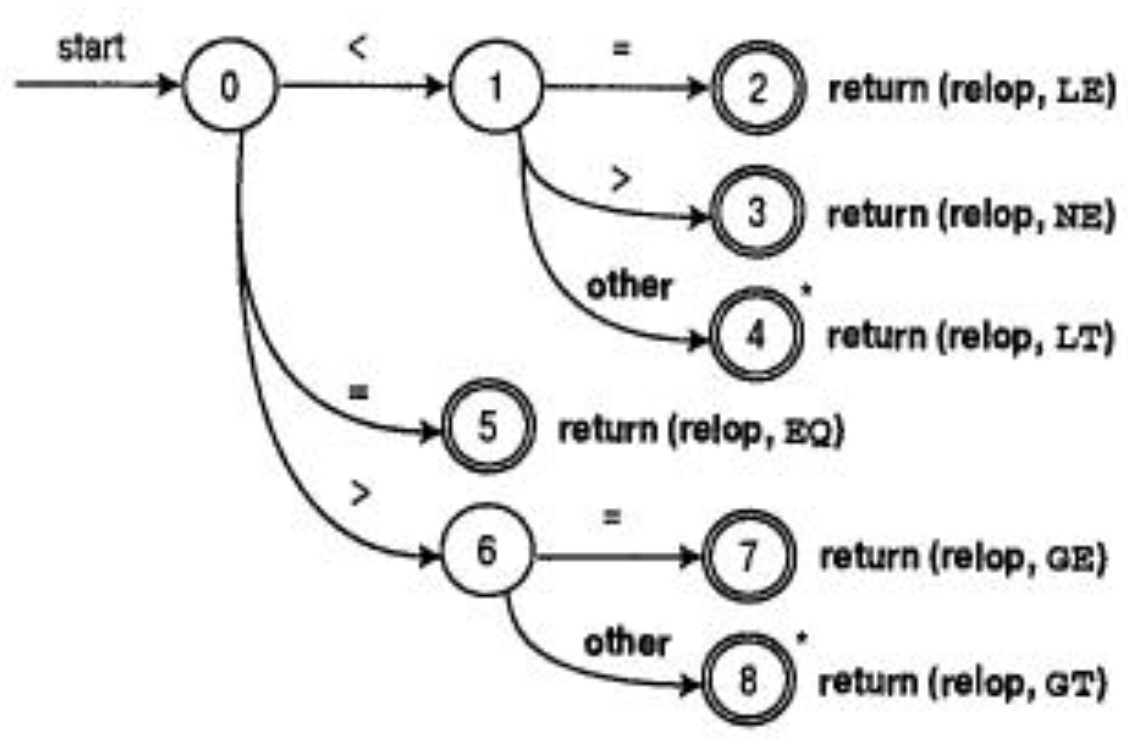
\includegraphics[height=0.5\textheight]{transitionDiagram.png}
        \end{center}
        \begin{outline}
            \1 Двойной кружок --- \textit{принимающее состояние}
            \1 Звёздочка --- вернуть последний символ во входной поток
        \end{outline}
    \end{frame}

    \begin{frame}{Как это закодить}
        $relop \rightarrow < | <= | = | <> | > | >=$
        \begin{columns}
            \begin{column}{0.5\textwidth}
                \begin{center}
                    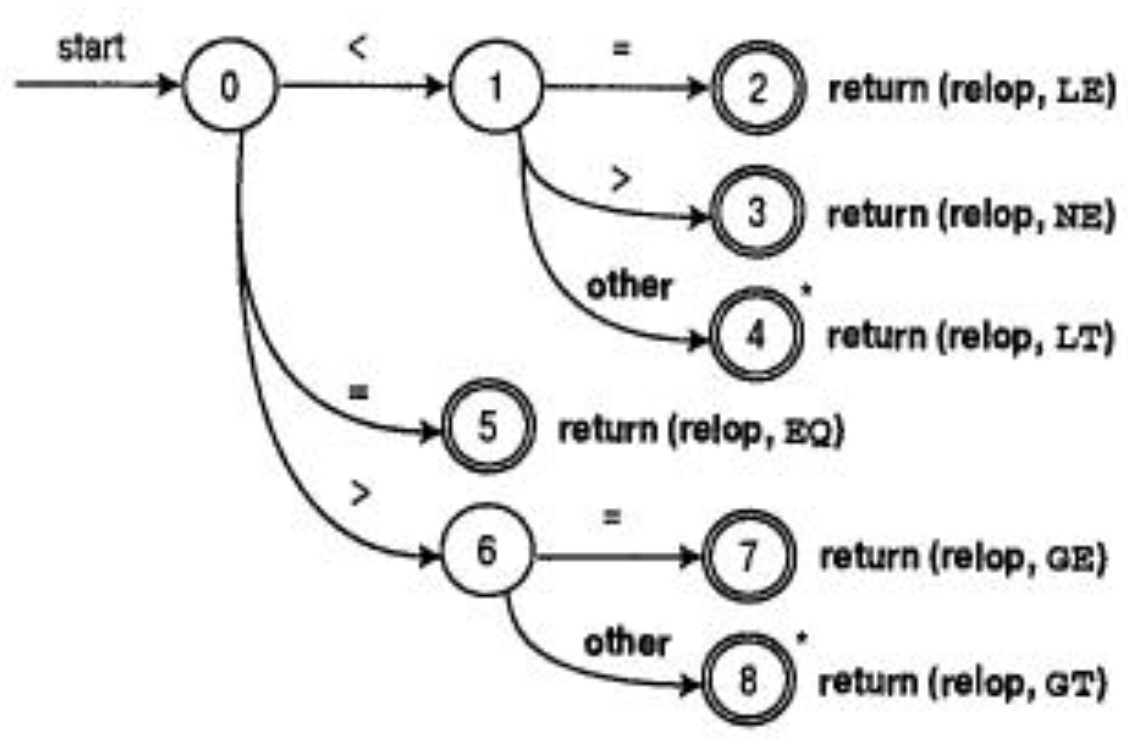
\includegraphics[width=0.9\textwidth]{transitionDiagram.png}
                \end{center}
            \end{column}
            \begin{column}{0.5\textwidth}
                \begin{center}
                    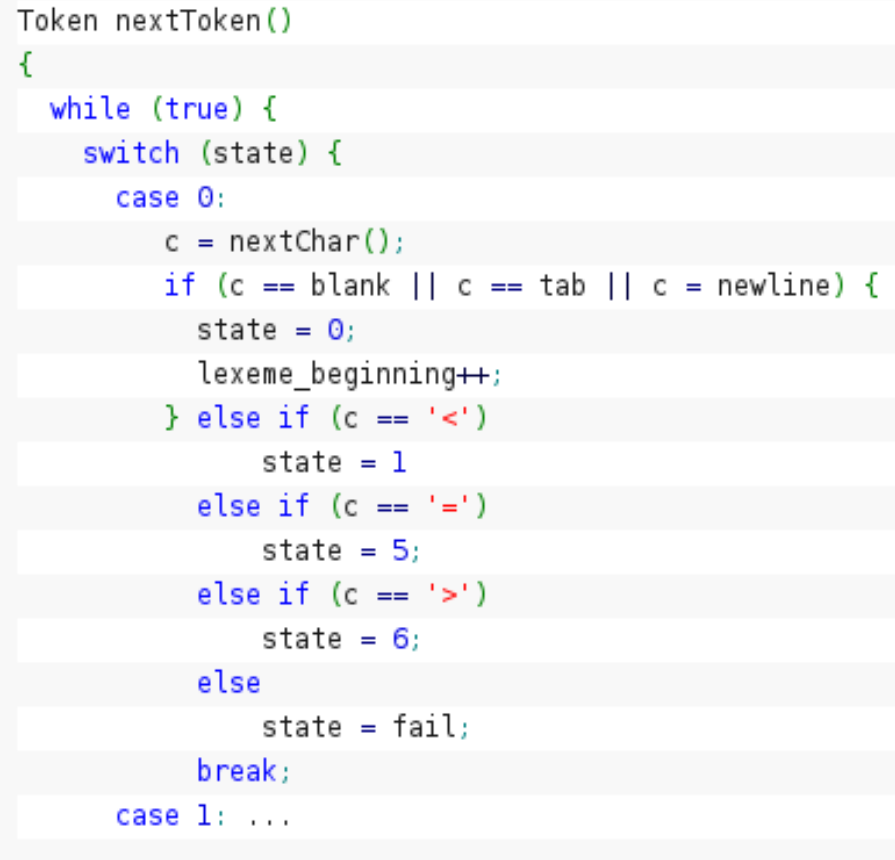
\includegraphics[width=0.9\textwidth]{lexerCode.png}
                \end{center}
            \end{column}
        \end{columns}
    \end{frame}

    \section{Автоматы}

    \begin{frame}{Конечные автоматы}
        \begin{outline}
            \1 Конечный автомат --- $(S, \Sigma, move, s_0, F)$
                \2 $S$ --- множество состояний
                \2 $\Sigma$ --- входной алфавит
                \2 move --- функция переходов
                \2 $s_0$ --- начальное состояние
                \2 $F$ --- множество допускающих состояний
            \1 Неформально автомат имеет состояние, в зависимости от которого может по-разному реагировать на входные символы (или события)
            \1 Применяются не только в лексическом анализе, но и в сетевых протоколах, пользовательских интерфейсах и т.д. и т.п.
            \1 Автомат принимает язык, если для любой строки языка после выполнения всех переходов он оказывается в допускающем состоянии
        \end{outline}
    \end{frame}

    \begin{frame}{ДКА и НКА}
        \begin{outline}
            \1 Детерминированный конечный автомат (ДКА) --- $move: S \times \Sigma \rightarrow S$
            \1 Недетерминированный конечный автомат (НКА) --- $move: 2^S \times \Sigma \cup \epsilon \rightarrow 2^S$
                \2 НКА может находиться в нескольких состояниях одновременно и делать переход одновременно в несколько разных состояний
                \2 Или, другая точка зрения --- он не знает, в каком именно состоянии сейчас находится
                \2 И есть эпсилон-переходы --- спонтанные переходы, без входного символа
        \end{outline}
    \end{frame}

    \begin{frame}{Пример НКА}
        Пусть есть язык, задаваемый регулярным выражением $a a^* \mid b b^*$. Тогда его принимает НКА:
        \begin{center}
            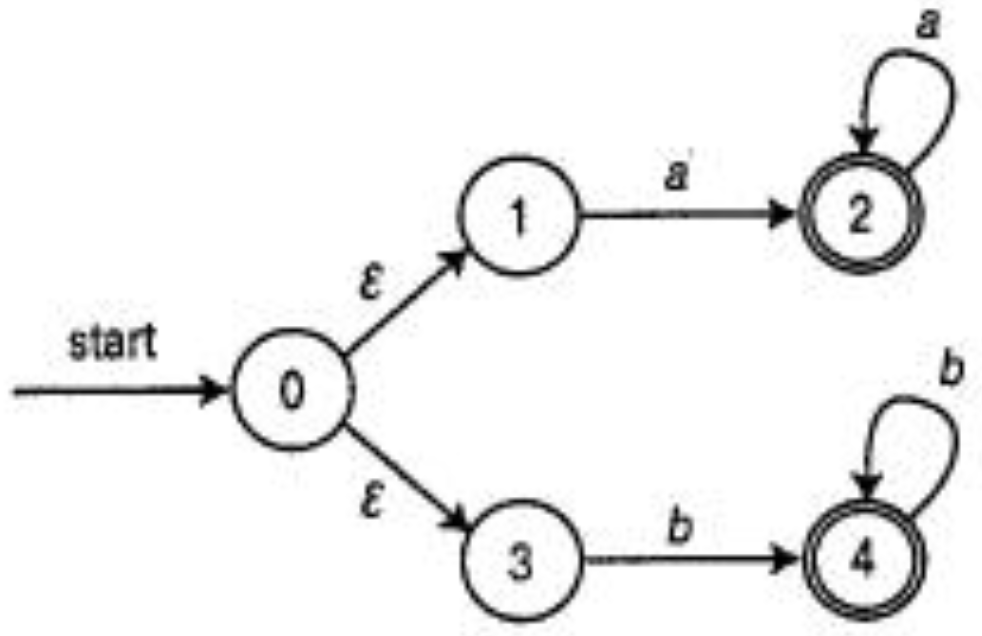
\includegraphics[height=0.6\textheight]{nfa.png}
        \end{center}
    \end{frame}

    \begin{frame}{Построение НКА по регулярному выражению}
        Теорема: по любому РВ можно построить НКА, принимающий язык РВ. Доказательство:
        \begin{center}
            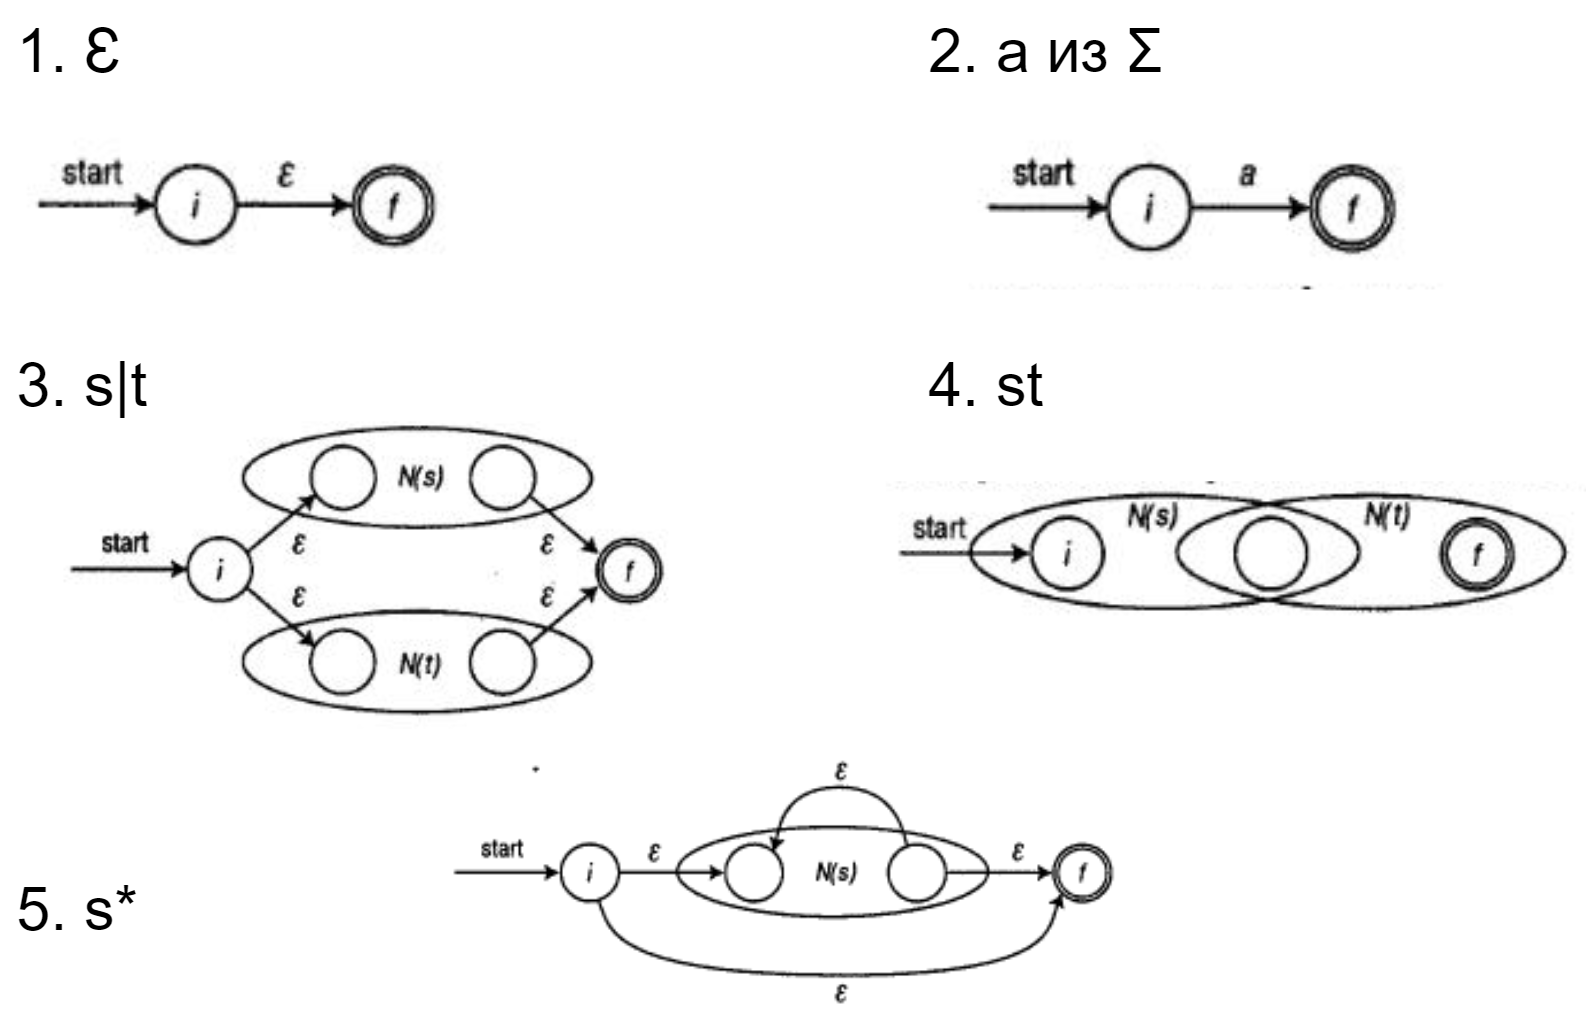
\includegraphics[height=0.6\textheight]{nfaByRegexp.png}
        \end{center}
    \end{frame}

    \begin{frame}{Моделирование НКА, таблица переходов}
        \begin{center}
            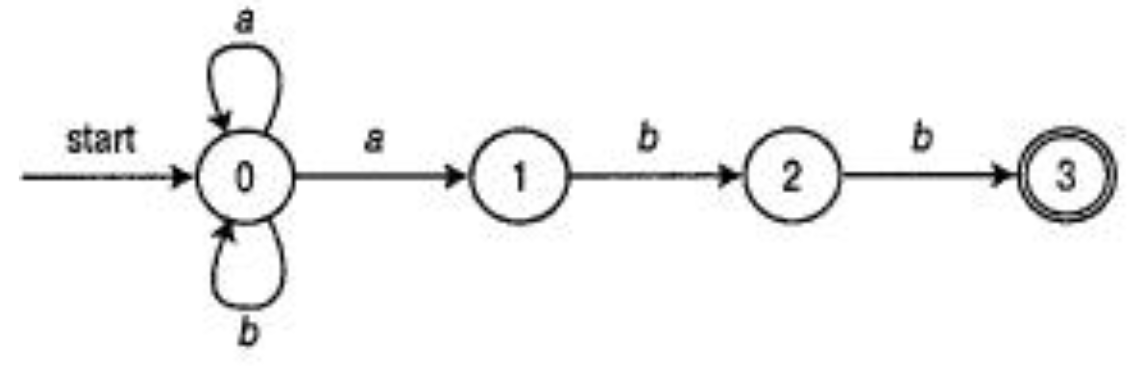
\includegraphics[width=0.8\textwidth]{abbNfa.png}
        \end{center}
        \begin{center}
            \begin{tabu} {| X[0.9 l p] | X[1 l p] | X[1 l p] |}
                \tabucline-
                Состояние              & a           & b        \\
                \tabucline-
                \everyrow{\tabucline-}
                0                      & $\{0, 1\}$  & $\{0\}$  \\
                1                      & ---         & $\{2\}$  \\
                2                      & ---         & $\{3\}$  \\
            \end{tabu}
        \end{center}
    \end{frame}

    \begin{frame}{Построение ДКА по НКА}
        Теорема: по любому НКА можно построить ДКА, принимающий в точности тот же язык (то есть НКА и ДКА эквивалентны друг другу в плане выразительности).

        Без доказательства.
    \end{frame}

    \begin{frame}{Пример}
        \begin{center}
            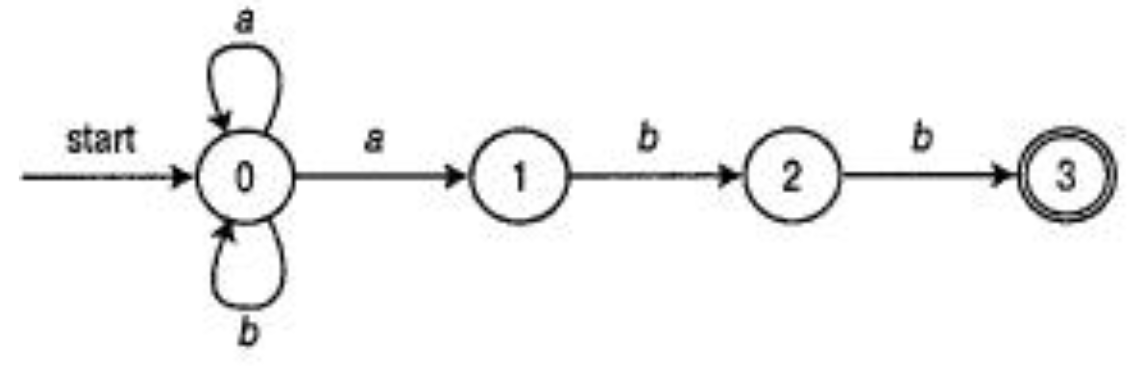
\includegraphics[width=0.7\textwidth]{abbNfa.png}
        \end{center}
        \begin{center}
            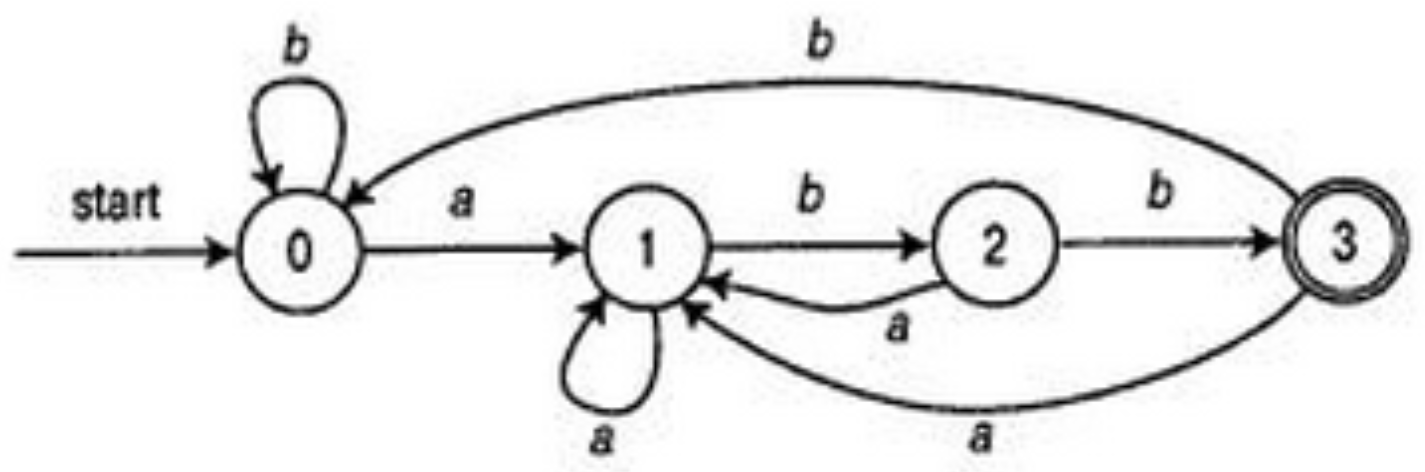
\includegraphics[width=0.7\textwidth]{abbDfa.png}
        \end{center}
    \end{frame}

    \begin{frame}{Моделирование ДКА}
        \begin{center}
            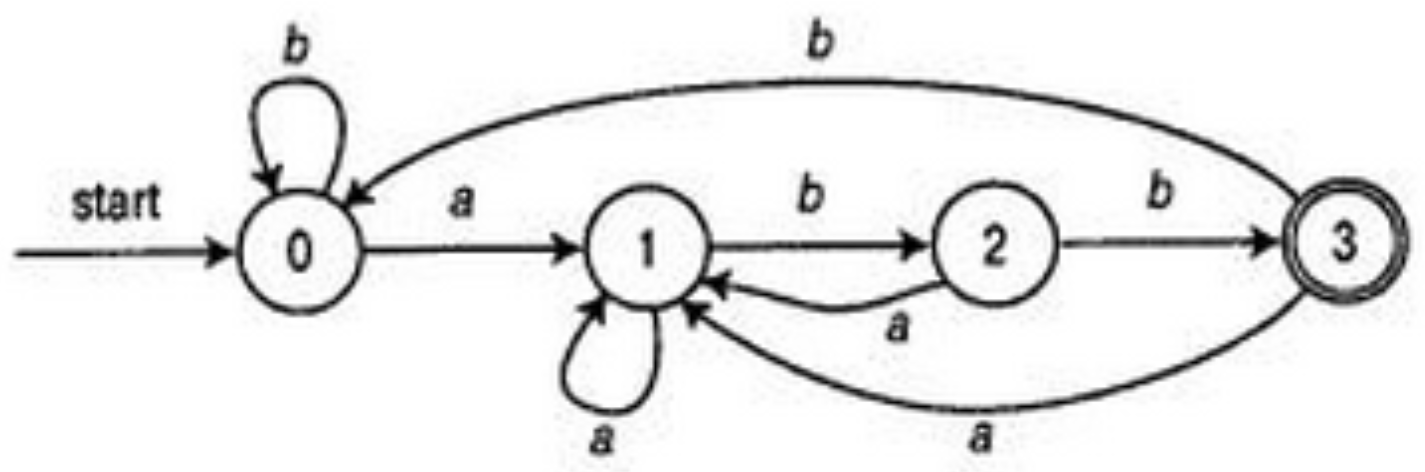
\includegraphics[width=0.7\textwidth]{abbDfa.png}
        \end{center}
        \begin{center}
            \begin{tabu} {| X[0.9 l p] | X[1 l p] | X[1 l p] |}
                \tabucline-
                Состояние              & a         & b  \\
                \tabucline-
                \everyrow{\tabucline-}
                0                      & 1         & 0  \\
                1                      & 1         & 2  \\
                2                      & 1         & 3  \\
                3                      & 1         & 0  \\
            \end{tabu}
        \end{center}
    \end{frame}

    \begin{frame}[fragile]{Как это выглядит в коде}
        \begin{outline}
            \1 switch-case вполне вариант
            \1 Интерпретировать таблицу состояний
                \2 Лучше, меньше кода и гибче
        \end{outline}
        \begin{minted}{pascal}
while c <> eof do begin
    s := move(s, c);
    c := nextchar();
end;
return (s in F);
        \end{minted}
    \end{frame}

    \begin{frame}{Материалы}
        \begin{columns}
            \begin{column}{0.5\textwidth}
                Книжка:

                А. Ахо, Р. Сети, Дж. Ульман, М. Лам. Компиляторы. Принципы, технологии, инструменты.
            \end{column}
            \begin{column}{0.5\textwidth}
                \begin{center}
                    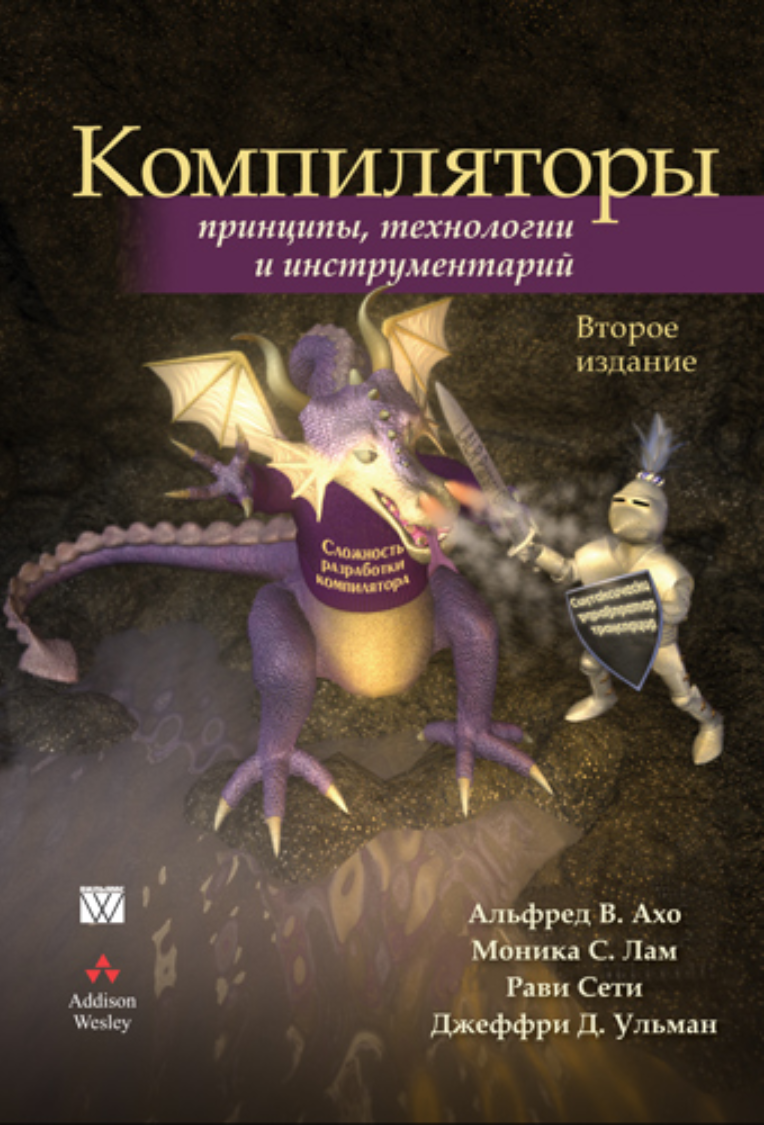
\includegraphics[width=0.38\textwidth]{compilersCover.png}
                \end{center}
            \end{column}
        \end{columns}

        Конструктор автоматов:
        \begin{outline}
            \1 Веб-версия: \url{https://spbu-se.github.io/WebAutomataConstructor}
            \1 GitHub: \url{https://github.com/spbu-se/WebAutomataConstructor}
            \1 Десктопная версия: \url{https://github.com/spbu-se/DesktopAutomataConstructor}
        \end{outline}
    \end{frame}

\end{document}